\chapter{Flutter}
\section{Introduzione}
\textbf{Flutter} è un framework sviluppato da Google che permette di realizzare delle applicazioni compilate nativamente per dispositivi mobili, Web e desktop a partire da un \textit{singolo codice sorgente}, scritto in \textit{Dart} \cite{flutter}. L'obiettivo è consentire agli sviluppatori di offrire app ad alte prestazioni naturali su piattaforme diverse.

\section{Struttura del framework}
\begin{figure}
	\begin{center}
		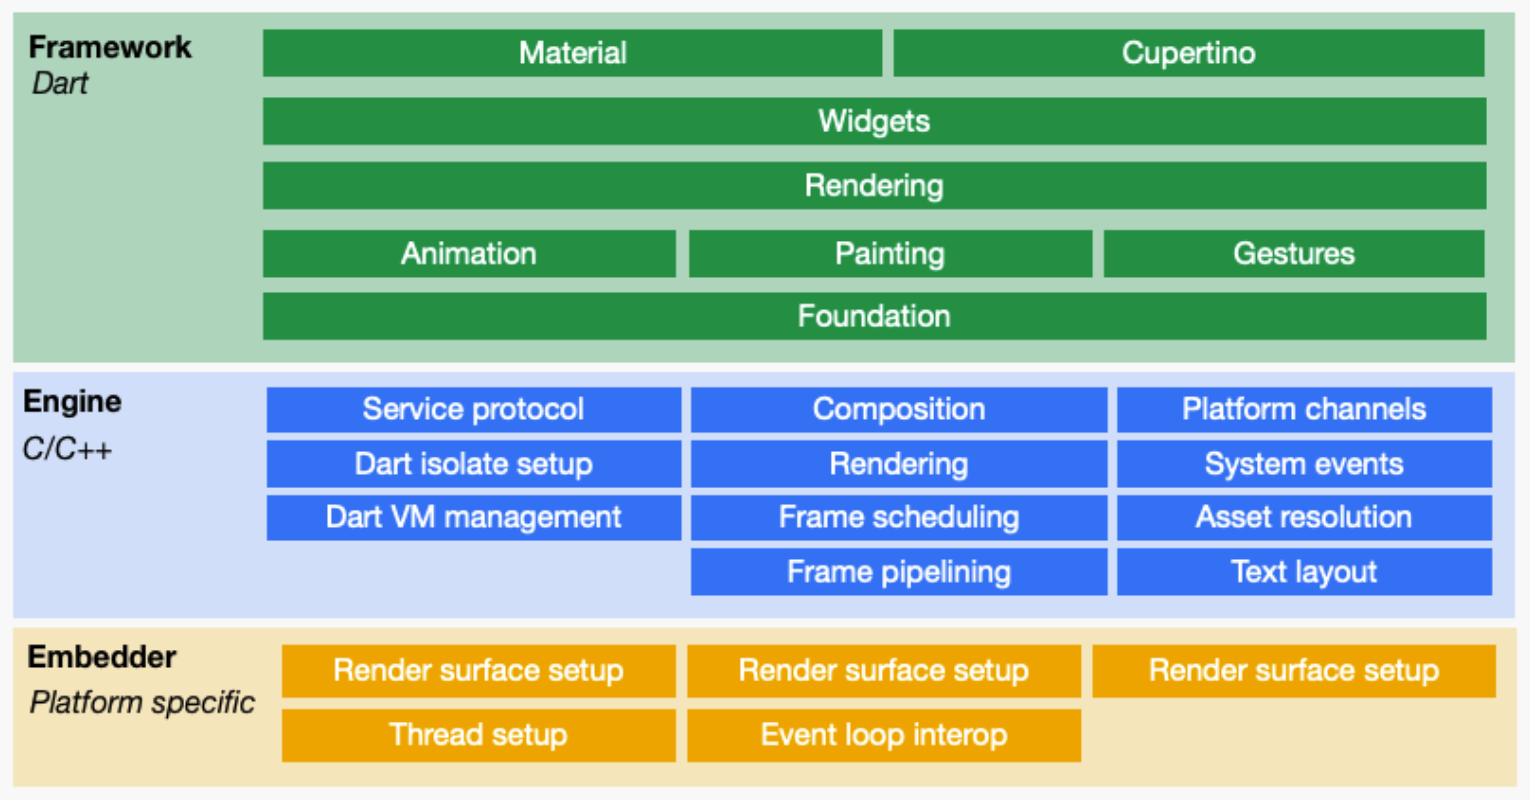
\includegraphics[scale=0.5]{architettura_framework_flutter}
		\caption[Architettura del framework Flutter]{Architettura del framework \cite{flutter_technical_overview}.}
		\label{figura:architettura_framework_flutter}
	\end{center}
\end{figure}

Il framework è strutturato a \textit{strati} con l'obiettivo di poter realizzare di più, scrivendo meno codice. È stato pensato per facilitare la stesura e la leggibilità del codice. 

Flutter si divide in:
\begin{enumerate}
	\item \textbf{Framework}: è lo strato superficiale realizzato in Dart. Vengono messe a disposizione librerie ed astrazioni necessarie per lo sviluppo dell'applicazione. In particolare è possibile notare il livello dedicato ai \textbf{Widget}, uno dei più importanti durante lo sviluppo. Sulla base di questo \textit{layer} è possibile definire altri due livelli: \textit{Material} e \textit{Cupertino}. Questi due strati implementano rispettivamente i componenti grafici secondo lo stile Android e iOS. È lo strato che viene per la maggior parte utilizzato dai programmatori durante lo sviluppo dell'applicazione. Gli sviluppatori possono creare dei nuovi componenti sulla base di quelli già forniti da Flutter o creare dei nuovi componenti ad-hoc;	
	\item \textbf{Engine}: realizzato in C++, permette di rendere le applicazioni prestanti ed efficienti. L'\textit{engine} include molti componenti di basso livello, fondamentali per il funzionamento del framework e per le sue operazioni di base. Tra questi troviamo il motore grafico \textit{Skia};
	\item \textbf{Embedder}: è il livello più basso dell’architettura e rappresenta il cuore dell'engine di Flutter. In questo strato vengono definiti gli \textit{embedder} specifici per le piattaforme, che hanno il compito di legare tra loro il rendering ai componenti della schermata nativa, alla gestione degli eventi di input e molto altro. Per implementare queste funzionalità, gli embedder interagiscono con l'engine (lo strato superiore) tramite delle API scritte in C/C++ di basso livello. Queste API non sono accessibili al programmatore, ma possono essere usate soltanto internamente da Flutter. Un altro componente importante di questo strato è la \textbf{shell} che ospita la \textit{macchina virtuale} di Dart. La shell è specifica per ogni piattaforma e offre un accesso alle API native della piattaforma in questione. Le shell implementano del codice specifico per permettere la gestione degli eventi del ciclo di vita dell’app, in base al sistema operativo di interesse.
\end{enumerate}

\subsection{Skia}
\textit{Skia} \cite{skia} è un software che permette di effettuare il \textit{rendering} dell'interfaccia grafica. Questa libreria è scritta in C++ e fornisce delle API comuni che funzionano su diverse piattaforme hardware e software (è utilizzata come motore grafico anche per \textit{Google Chrome}).

\section{Widget}
\textit{"Everything is a widget"} è il motto che più rappresenta Flutter \cite{flutter_technical_overview}.
I \textbf{Widget} sono i mattoni fondamentali dell'interfaccia utente dell'applicazione. I Widget sono tutti quegli oggetti che vengono visualizzati a schermo, con cui l'utente può interagire. I Widget, una volta dichiarati, sono \textit{immutabili}. Altri framework separano i concetti di viste, controller di visualizzazione, layout ed altre proprietà. Flutter invece raggruppa tutti questi concetti in un'unica rappresentazione, infatti, un Widget può definire:
\begin{enumerate}
	\item Una caratteristica del \textit{layout} (ad esempio, il \textit{padding});
	\item Un elemento \textit{stilistico} (ad esempio, il \textit{colore});
	\item Un elemento che va a costituire la \textit{struttura} dell'interfaccia grafica (ad esempio, un \textit{bottone}).
\end{enumerate}

Tutti i Widget che vengono utilizzati per la realizzazione della UI costituiscono una gerarchia basata sulla \textbf{composizione}. Ogni Widget eredita le proprietà dell'oggetto genitore, non esiste un Widget che sia separato da questa gerarchia. Essendo i Widget immutabili, vi è uno specifico meccanismo per gestire gli eventi. Quando l'interfaccia grafica deve essere aggiornata a seguito di un'interazione con l'applicazione, il framework viene informato di \textit{sostituire} un Widget della gerarchia (\textbf{Widget tree}) con un nuovo Widget. Il nuovo Widget può essere lo stesso di quello precedente ma con un nuovo contenuto oppure può essere un Widget differente. Quindi il framework opera un confronto tra il vecchio ed il nuovo Widget: se nota delle differenze tra i due, allora imposta il nuovo Widget, altrimenti lascia il Widget così com'è. Così facendo, si prevengono eventuali \textit{reload} inutili della UI, aggiornando la UI soltanto quando è necessario.

La composizione dei Widget è molto \textbf{flessibile}: c'è molta libertà nel comporre i vari Widget per creare degli elementi grafici \textit{personalizzati} e \textit{riusabili} in parti differenti dell'applicazione.

È rilevante precisare che il team di sviluppo di Flutter ha voluto realizzare un software differente dagli altri framework cross-platform presenti nel mercato: con Flutter è possibile personalizzare il \textbf{singolo pixel} dell'applicazione. Ai programmatori e ai designer è concessa la piena libertà nella personalizzazione della UI. Tale caratteristica permette a questo framework di differenziarsi da tutti gli altri. In particolare, diversamente da Flutter, \textit{React Native} (il principale competitor sviluppato da \textit{Facebook}) utilizza gli elementi grafici nativi che offre il sistema operativo. Ovvero, il team di React Native ha sviluppato delle API per interagire con tali componenti. Invece, nel caso di Flutter, tutti i componenti grafici sono stati completamente ridisegnati, appunto intervenendo su ogni singolo pixel. Il vantaggio di React Native è che se il sistema operativo apporta una modifica ad un componente grafico, il framework non deve essere aggiornato. Nel caso di Flutter, il team di sviluppo invece deve ridisegnare il componente e pubblicare un aggiornamento del framework. Tuttavia, Flutter lascia un'ampia libertà e flessibilità nella realizzazione degli elementi grafici, mentre React Native risulta essere più limitato da questo punto di vista, oltre ad avere la necessità di un \textit{bridge} per interagire con i componenti grafici, causando l'introduzione di \textit{overhead}.

\subsection{Classificazione dei Widget}
I Widget possono essere classificati in due categorie: possono essere \textbf{Stateful} o \textbf{Stateless}. Questa suddivisione nasce per motivi di efficienza. Come è stato accennato precedentemente, sulla base di un evento, il framework valuta se sostituire o meno un Widget. Tuttavia nell'interfaccia grafica è possibile trovare degli elementi che non vengono mai modificati durante tutto il ciclo di vita dell'applicazione: questi elementi possono essere bottoni, icone, testi ed altro ancora. Pertanto, questi Widget possono essere dichiarati \verb|Stateless|, ovvero, non necessitano di possedere uno \textbf{stato} che può cambiare nel tempo. Quindi queste tipologie di Widget, una volta \textit{renderizzate} dal framework, non vengono più aggiornate, ottenendo così delle performance migliori. I Widget vengono dichiarati \verb|Stateful| quando l'utente può interagire con loro, cambiando il loro \textit{stato}. Quando lo stato cambia, il framework si occupa di apportare le dovute modifiche, che possono essere, ad esempio, l'aggiornamento di un componente o l'aggiornamento di una variabile interna alla classe. Lo stato di un Widget è memorizzato in un oggetto di tipo \verb|State<T>|, in modo da mantenere separato lo stato del Widget dalla sua rappresentazione grafica. Quando lo stato del Widget cambia, l'oggetto \verb|State<T>| chiama il metodo \verb|setState()|, eseguendo il suo contenuto. Tuttavia, l'utilizzo del metodo \verb|setState()| comporta ad introdurre della business logic nella parte dedicata alla realizzazione dell'interfaccia grafica. Pertanto, per ovviare a questa problematica, viene sfruttata la \textit{programmazione reattiva}, presentata nel capitolo relativo all'introduzione al linguaggio Dart.

Di seguito, si illustra qual è la struttura di base per creare un \verb|Stateful| Widget e un \verb|Stateless| Widget:
\begin{enumerate}
	\item \textbf{Stateful}:
\lstset{numbers=left, % vogliamo numerare le righr
  numberstyle=\tiny, % i numeri sono piccoli
  basicstyle=\ttfamily, % usiamo il carattere dattilografico
  columns=fullflexible, % niente emulazioni di allineamento
  backgroundcolor=\color{lightgray}, % colore di sfondo
  language=Java, % linguaggio usato
  }
\begin{lstlisting}
class MyButton extends StatefulWidget {
	@override
 	_MyButtonState createState() => _MyButtonState();
}

class _MyButtonState extends State<MyButton> {
	@override
	Widget build() {
		// Build your own Widget 
		// by composing other Widgets
		return ...;
	}
}
\end{lstlisting}
	\item \textbf{Stateless}:
\begin{lstlisting}
class MyIcon extends StatelessWidget {
	@override
	Widget build() {
		// Build your own Widget 
		// by composing other Widgets
		return ...;
	}
}
\end{lstlisting}
\end{enumerate}

\subsection{Costruzione dei Widget}
\begin{figure}
	\begin{center}
		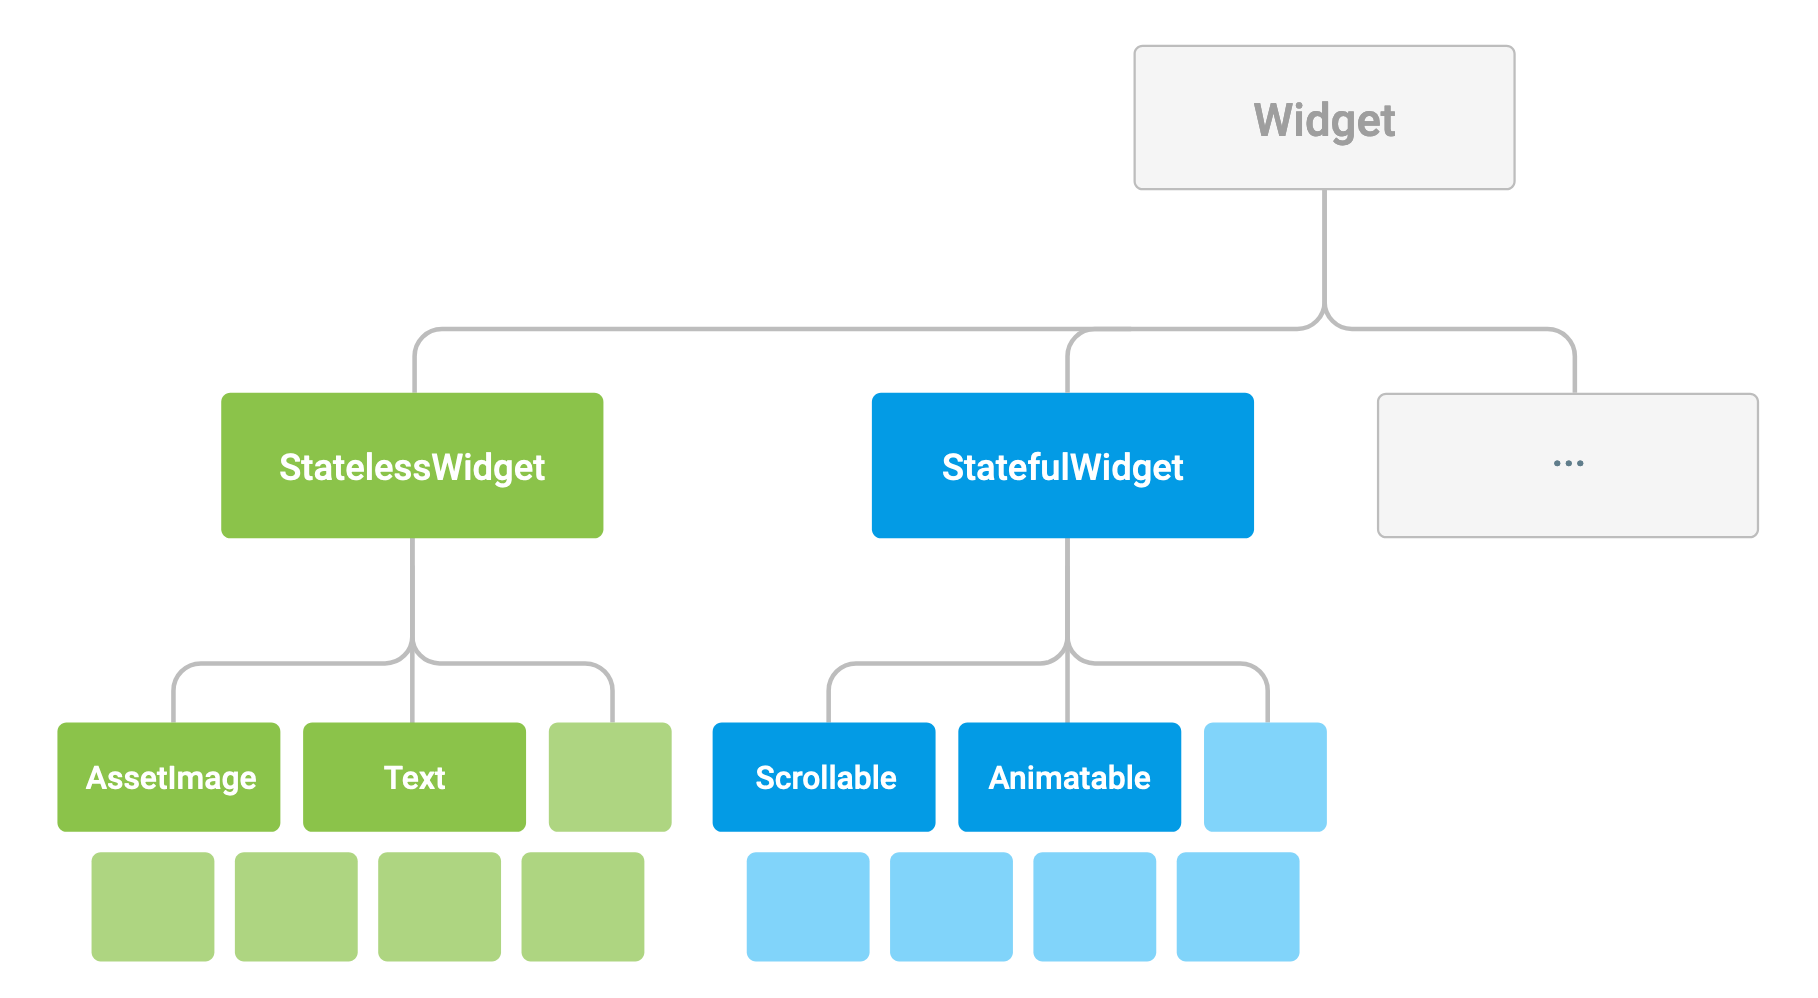
\includegraphics[scale=0.4]{stateful_stateless}
		\caption[Widget Stateful e Stateless]{Un esempio semplificato di un \textit{Widget tree} \cite{flutter_technical_overview}.}
		\label{figura:stateful_stateless}
	\end{center}
\end{figure}

Per costruire il Widget, il framework chiama il metodo \verb|build()|, presente sia nella classe \verb|Stateful| che nella classe \verb|Stateless|. Questo metodo restituisce un albero di Widget (\textit{Widget tree}). Se ci poniamo nella radice di questo albero, verrà restituito tutto l'albero dei Widget dell'applicazione; se ci poniamo in un nodo interno di questo albero, verrà restituito un sottoalbero del Widget tree. L'albero rappresenta l'interfaccia utente, realizzata per composizione con i vari Widget. A partire dalla radice, il framework chiama \textbf{ricorsivamente} il metodo \verb|build()| per ciascun Widget, fino a quando non si arriva alle foglie dell'albero, ovvero, si arriva a costruire dei Widget elementari, che non sono più costituiti da altri Widget. Un esempio semplificato di un Widget tree è illustrato nella Figura 5.2.

La creazione di un Widget dovrebbe essere \textit{priva di effetti collaterali}. A seguito di un cambiamento dello stato dell'applicazione, il framework confronta la struttura costruita precedentemente con la struttura costruita in quel preciso istante, per determinare quali modifiche devono essere apportate all'interfaccia utente. Questo confronto automatizzato risulta essere efficace, consentendo la realizzazione di applicazioni interattive e prestanti. 

L'utilizzo del metodo \verb|build()| permette di focalizzarsi sul come costruire un Widget per composizione, tralasciando la complessità dell'aggiornamento della UI da uno stato ad un altro.

\section{State Management}
L'utilizzo della programmazione reattiva porta a gestire in maniera differente i dati che devono essere comunicati tra i vari componenti. Nella comunità di Flutter, questo è un tema sempre molto discusso, da cui fuoriescono diverse soluzioni e possibili architetture per gestire in modo efficiente la \textit{gestione dello stato} (\textit{state management}). Una qualsiasi modifica, come la ricezione di un messaggio o l'interazione dell'utente con l'app, può essere intesa come una variazione dello stato dell'applicazione. Questo aspetto è di fondamentale importanza in quanto è una caratteristica intrinseca del framework: pertanto, questo tema deve essere affrontato ampiamente, andando ad analizzare la documentazione fornita dalla comunità di Flutter. Se lo \textit{state management} non viene gestito correttamente durante lo sviluppo dell'applicazione, non solo si possono ottenere delle inefficienze dal punto di vista delle prestazioni, ma anche delle vere e proprie problematiche nella comunicazione dei cambiamenti di stato, che possono causare, per esempio, la mancata ricezione di alcuni dati. Nel contesto d'uso in cui l'applicazione deve far parte, è necessario porre molta attenzione nella ricerca e nello sviluppo di un'architettura che riesca a gestire correttamente lo \textit{state management}.

Di seguito vengono elencate le diverse soluzioni ed architetture proposte fino ad ora, sia dal team di Flutter che dalla comunità.

\subsection{setState}
Questo è l'approccio di gestione dello stato più semplice presente in Flutter. Tramite la funzione \verb|setState()| è possibile indicare nel suo corpo tutte le operazioni che modificano il valore di un qualche oggetto dell'applicazione. Questo oggetto è condiviso da più Widget e pertanto la modifica di tale deve avvenire all'interno del metodo \verb|setState()| in modo da forzare il framework ad aggiornare i rispettivi Widget.

I vantaggi sono la facilità di utilizzo e la facilità di comprensione del meccanismo. Tuttavia, quando l'applicazione cresce di complessità, questo approccio risulta essere molto limitante. Gli altri svantaggi sono:
\begin{enumerate}
	\item Non è possibile gestire degli stati che devono persistere tra le sessioni;
	\item L'utilizzo di questo approccio rende il processo di manutenzione molto più laborioso e complicato in quanto lo stato viene sparso in varie zone dell'applicazione;
	\item Si inserisce nel codice dedicato all'interfaccia grafica, mescolando UI e business logic;
\end{enumerate}

Questo approccio è consigliato per la realizzazione di piccole applicazioni e che in futuro non verrano ampliate.

\subsection{InheritedWidget}
\verb|InheritedWidget| è un Widget che non mostra nulla a livello grafico ma permette di salvare dei dati al suo interno e di propagarli nel Widget tree a lui sottostante. I Widget dell'albero possono accedere ai dati del \verb|InheritedWidget| tramite il metodo \verb|InheritedWidget.of(context)|. Questo approccio è alla base del pattern Provider e viene ampiamente utilizzato anche per la creazione di molti componenti di default di Flutter.

\newpage

\subsection{Scoped Model}
Lo \verb|Scoped Model| è un approccio basato su \verb|InheritedWidget| e offre un modo, leggermente migliore, per accedere, aggiornare e mutare lo stato. Permette di passare facilmente un \verb|Model| di dati da un Widget genitore ai suoi discendenti. Inoltre, ricostruisce anche tutti i \textit{child} che utilizzano tale modello, nel momento in cui questo viene aggiornato. Così facendo, potrebbero sorgere delle problematiche relative alle prestazioni, a seconda di quanti \verb|ScopedModelDescendants| ha un modello. I \verb|ScopedModelDescendants| vengono ricostruiti ogni qual volta è presente un nuovo aggiornamento dello stato. Questo problema può essere risolto decomponendo lo \verb|ScopedModel| in più modelli, in modo da ottenere delle dipendenze più precise. 

Specificando il flag \verb|rebuildOnChange| su \verb|false|, viene risolto il problema, in quanto si va a specificare quale Widget necessita di essere ricostruito all'aggiornamento dello stato.

\subsection{Redux}
\begin{figure}
	\begin{center}
		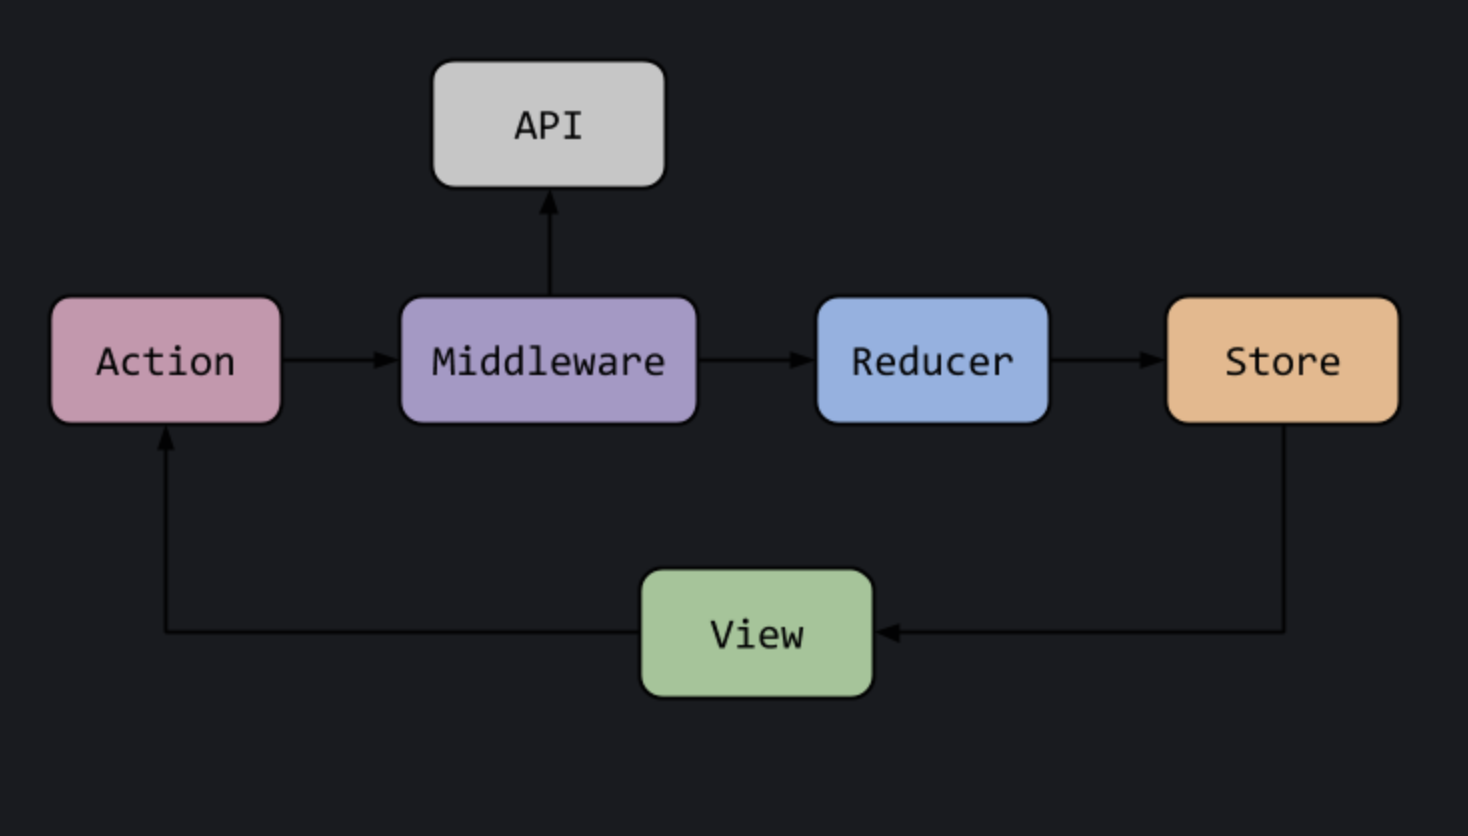
\includegraphics[scale=0.4]{redux}
		\caption[State management - Redux]{Il pattern architetturale Redux.}
		\label{figura:redux}
	\end{center}
\end{figure}

\textbf{Redux} è un'architettura nella quale è presente un unico flusso unidirezionale dei dati che semplifica lo sviluppo, la manutenzione e il test delle applicazioni \cite{redux}.

È una nota libreria JavaScript ampiamente utilizzata in React. Grazie al suo successo, è stato effettuato un \textit{porting} della libreria per Flutter.

\subsection{Provider e BLoC}
Questi due pattern architetturali verranno descritti ampiamente nel capitolo successivo, in quanto sono i due principali metodi utilizzati per la realizzazione dell'architettura complessiva dell'applicazione.

\section{Hot Reload}
Questa rappresenta una delle funzionalità più apprezzate dagli sviluppatori Flutter. Google tentò più volte di implementare \textit{Instant Run} per lo sviluppo di applicazioni per Android, ma con scarsi successi.

Nella fase di sviluppo di un'applicazione, Flutter utilizza il compilatore \textit{JIT}. L'\textit{hot reload} permette di ricaricare e di continuare l'esecuzione del codice, in pochi decimi di secondo. Lo stato dell'applicazione rimane inalterato tra un \textit{reload} e l'altro quando possibile: se avviene un aggiornamento dal punto di vista grafico, allora lo stato rimane inalterato; se invece l'aggiornamento apportato riguarda una modifica fatta a livello di business logic, allora è possibile che lo stato venga alterato. In quel caso sarà necessario ricompilare l'applicazione per ripristinare uno stato consistente. 

Questa funzionalità accelera i tempi di sviluppo dell'interfaccia grafica in quanto vengono eliminati tutti i tempi di attesa, dal momento in cui viene avviata la nuova compilazione fino al suo termine. Pur sembrando irrisori, la somma di tutti questi tempi morti comporta a risparmiare molto tempo durante l'intero processo di sviluppo e anche durante la fase di \textit{debugging} \cite{hot_reload}.

\section{Fuchsia}
\begin{figure}
	\begin{center}
		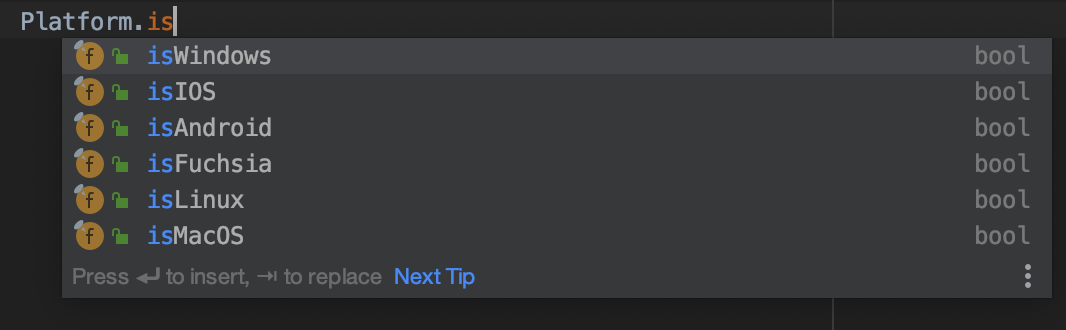
\includegraphics[scale=0.7]{fuchsia_multipiattaforma}
		\caption[Flutter - Supporto sistemi operativi]{Già da diverse verisioni dell'SDK di Flutter, sono presenti alcuni suggerimenti per il futuro supporto di Fuchsia (la versione di Flutter in questione è la \textit{1.12.13+hotfix.9} del canale stabile e la versione di Dart è la \textit{2.7.2}).}
		\label{figura:fuchsia_multipiattaforma}
	\end{center}
\end{figure}

Lo sviluppo di questo framework fa parte di un contesto molto più grande di quello attuale. Negli ultimi anni Google ha iniziato a sviluppare un nuovo sistema operativo denominato \textbf{Fuchsia} \cite{fuchsia} \cite{fuchsia_wikipedia}. A differenza dei precedenti sistemi operativi, come Android e Chrome OS, che si basano su kernel \textit{Linux}, Fuchsia si basa su un nuovo \textit{microkernel} denominato \textbf{Zircon}, derivato da \textit{Little Kernel (LK)}, progettato per funzionare su qualsiasi dispositivo. In particolare è stato progettato per funzionare su smartphone e computer moderni, con processori veloci, quantità molto alte di memoria RAM e con periferiche arbitrarie per il calcolo computazionale.

Flutter diventerà il principale framework di sviluppo per le applicazioni di Fuchsia. Per essere più precisi, l'SDK di Flutter sarà nativamente supportato dal futuro sistema operativo (si veda Figura 5.3).

Una delle proprietà più rilevanti di Fuchsia che è possibile notare è la capacità di adattare l'interfaccia grafica a seconda del dispositivo in cui viene eseguito, tutto in maniera estremamente semplice. L'obiettivo di Google è un obiettivo molto ambizioso, intrapreso recentemente da diverse aziende tecnologiche come Mircrosoft, Samsung ed Apple. In particolare:
\begin{enumerate}
	\item Microsoft ha tentato l'unificazione con la \textit{Universal Windows Platform} (UWP), progetto naufragato a causa della rimozione del supporto a \textit{Windows Mobile}. L'obiettivo era quello di realizzare applicazioni universali che potessero essere eseguite su Windows 10, Windows 10 Mobile e Xbox One;
	\item Samsung ha avviato \textit{Samsun DeX}: collegando il proprio smartphone al ad un monitor e ad una tastiera è possibile utilizzarlo tramite un'interfaccia che si adatta alle dimensioni di un monitor;
	\item Apple ha presentato \textit{Apple Catalyst}, un software che permette di creare applicazioni che possono essere eseguite sia su Mac che iPad.
\end{enumerate}

Osservando tutte queste iniziative  avviate dalle più grandi aziende tecnologiche al mondo, è facile intuire che il futuro sarà l'unificazione dei dispositivi mobili, tablet e desktop dal punto di vista delle applicazioni.

Nell'ultimo periodo, Fuchsia è stato testato su un insieme di dispositivi molto differenti tra loro: è stato testato su uno smartphone Huawei, su un Google Nest Hub \cite{fuchsia_google_nest_hub}, Chromebook ed altri.

\section{Ciclo di vita delle applicazioni}
Il \textit{ciclo di vita} di un'applicazione Flutter è leggermente differente sia dal ciclo di vita di un'app Android che iOS. Il motivo è che essendo un framework cross-platform, deve riuscire ad interagire con entrambi i sistemi operativi. Pertanto, risulta necessario avere un ciclo di vita comune a tutti i sistemi operativi. Gli eventi nel ciclo di vita di un'app in Flutter sono:
\begin{enumerate}
	\item \textbf{inactive}: l’applicazione è inattiva e non riceve input dall’utente. Questo evento funziona solo per iOS in quanto non esiste un evento corrispondente in Android;
	\item \textbf{paused}: l’applicazione non è momentaneamente visibile all’utente, non risponde ai suoi input ed è eseguita in background (corrisponde all'evento \verb|onPause()| di Android);
	\item \textbf{resumed}: l’applicazione è visibile e risponde all’input dell’utente (corrisponde all'evento \verb|onPostResume()| di Android);
	\item \textbf{suspending}: l’applicazione è momentaneamente sospesa. Equivale all'evento \verb|onStop()| di Android. Non esiste un evento corrispondente su iOS.
\end{enumerate}

Flutter non mette a disposizione molti metodi per il controllo del ciclo di vita. Il motivo è che ci sono poche argomentazioni valide per osservare il ciclo di vita dal punto di vista di Flutter e quindi tali metodi vengono nascosti allo sviluppatore. Questi metodi vengono eseguiti internamente dal framework. Nel caso fosse strettamente necessario dover osservare il ciclo di vita per poter acquisire o rilasciare delle risorse, è preferibile farlo nativamente.

\section{Pacchetti}
In precedenza è stato introdotto il \textit{Pub} di Dart, ovvero, una raccolta di pacchetti open source disponibili anche per Flutter. In un'applicazione Flutter, questi pacchetti devono essere annotati dal programmatore su un particolare file: \textbf{pubspec.yaml}. Questo file è presente in qualsiasi progetto Flutter, fin dal momento della sua creazione. In questo file sono contenute:
\begin{enumerate}
	\item Tutte le dipendenze dell'applicazione;
	\item I percorsi degli \textit{asset} (ad esempio: icone, immagini, file JSON, font);
\end{enumerate}

Per importare nel progetto un pacchetto, è sufficiente scrivere sotto la voce \verb|dependencies| il nome e la versione del pacchetto (ad esempio, \\ \verb|url_launcher: ^5.4.7|\cite{pacchetto_url_launcher}). Successivamente sarà necessario lanciare il comando \verb|flutter pub get| per poter scaricare il pacchetto desiderato. Non è necessario effettuare il download manuale, è sufficiente indicare il nome e la versione del plugin e il sistema provvederà a scaricarlo e ad integrarlo automaticamente nel progetto.

\section{Vantaggi e svantaggi di Flutter}
In conclusione ai capitoli relativi a Dart e Flutter, si elencano alcuni vantaggi e svantaggi dell'utilizzo congiunto di questo linguaggio e di questo framework, sulla base anche dell'esperienza ottenuta durante lo sviluppo del progetto.

I vantaggi di utilizzare Flutter come framework di sviluppo sono:
\begin{enumerate}
	\item \textbf{Hot Reload}: funzionalità che consente di visualizzare le modifiche apportate al codice quasi in tempo reale, senza necessità di riavviare l'applicazione. Le modifiche apportate vengono inserite nell'applicazione in esecuzione e Flutter ricostruisce automaticamente il Widget tree in modo che tali modifiche vengano visualizzate in tempo reale;
	\item \textbf{Prestazioni}: Flutter non utilizza alcun \textit{bridge} in JavaScript per visualizzare in modo reattivo l'applicazione, come nel caso di React Native. L'applicazione quindi risulterà più prestante e veloce;
	\item \textbf{Programmazione reattiva}: permette di non fare uso del metodo \\ \verb|setState()|, migliorando la \textit{riusabilità del codice}, in quanto rende possibile la separazione della business logic dall'interfaccia grafica. Inoltre, migliora le prestazioni dell’applicazione, poiché evita di ridisegnare un Widget e l’intero Widget tree ad ogni modifica apportata. Le modifiche vengono propagate mediante gli \verb|Stream|.
\end{enumerate}

Di seguito, si elencano gli svantaggi dell'utilizzo di Flutter e, più in generale per alcuni punti, dei framework cross-paltform:
\begin{enumerate}
	\item \textbf{Dart}: diversamente da altri framework che utilizzano dei linguaggi già affermati nel mondo dello sviluppo software (JavaScript nel caso di React Native e C\# nel caso di Xamarin), imparare un nuovo linguaggio comporta comunque il dover superare una certa \textit{curva di apprendimento}, seppur bassa. La curva di apprendimento è bassa ed è dovuta alla vicinanza di Dart a linguaggi come JavaScript e Java, che semplificano l'apprendimento di tale linguaggio.
	\item \textbf{Multipiattaforma}: con un accezione negativa, non è possibile sviluppare delle applicazioni che devono implementare delle funzionalità che sfruttano dei particolari servizi offerti dal sistema operativo;
	\item \textbf{Dimensioni dell'applicazione}: non possono essere create delle applicazioni di dimensioni inferiori ai 4 MB. Il motivo riguarda la natura stessa di Flutter: nel codice dell'applicazione devono essere inclusi tutti i Widget necessari, in quanto il framework non utilizza i componenti grafici offerti dal sistema operativo;
	\item \textbf{Programmazione reattiva}: non sempre è possibile utilizzare la programmazione reattiva, spesso rende difficoltosa la leggibilità del codice, specialmente se la struttura dei Widget implementati è complessa.
\end{enumerate}

\section{Confronto con React Native}

\subsection{Introduzione a React Native}
\textbf{React Native} è un framework JavaScript per lo sviluppo di applicazioni mobili che permette di effettuare il rendering nativo sia per iOS che per Android. Questo framework si basa su \textit{React}, la libreria JavaScript di Facebook per la creazione di interfacce utente Web. Il motivo di questa scelta risulta essere molto astuta: Facebook può coinvolgere gli sviluppatori, che già conoscono la versione Web, verso lo sviluppo di applicazioni multipiattaforma, senza dover far imparare  agli sviluppatori delle nuove logiche ed una nuova architettura per realizzare applicazioni mobile. Gli sviluppatori dovranno fare un minimo sforzo per capire in che modo il framework interagisce con i dispositivi.

Analogamente a \textit{React.js} (la libreria Web), le applicazioni React Native sono scritte usando una combinazione di JavaScript e XML, noto come \textit{JSX}. Quindi, il \textbf{bridge} nativo di React invoca le API di rendering native in Objective-C (per iOS) e in Java (per Android). Pertanto, l'applicazione eseguirà il rendering utilizzando i componenti grafici già presenti nel sistema operativo, senza effettuare visualizzazioni Web. React Native espone anche le interfacce JavaScript per le API della piattaforma, quindi le applicazioni React Native possono accedere a funzionalità del dispositivo come la videocamera del telefono o la posizione dell'utente.

\subsection{Confronto}

\subsubsection{Linguaggio di programmazione utilizzato}
\textbf{React Native} utilizza JavaScript per creare le applicazioni. JavaScript è un linguaggio molto popolare nello sviluppo di applicazioni Web. Con React Native, gli sviluppatori Web possono creare delle applicazioni mobili, aggiungendo poche conoscenze basilari.

\textbf{Flutter} utilizza \textit{Dart} come linguaggio per scrivere le applicazioni. È stato introdotto da Google e il suo uso è limitato a questo framework. La sintassi Dart è di facile comprensione per gli sviluppatori JavaScript o Java, in quanto supporta la maggior parte dei concetti orientati agli oggetti. Inoltre il linguaggio è provvisto di una buona documentazione.

\textit{JavaScript} è ampiamente utilizzato dalla maggior parte degli sviluppatori Web: di conseguenza è facile adottare il framework React Native. Nonostante Dart abbia delle ottima funzionalità e caratteristiche, è usato raramente ed è meno conosciuto nella comunità degli sviluppatori.

\subsubsection{Architettura}
L'architettura di \textbf{React Native} si basa fortemente sull'architettura dell'ambiente di runtime Javascript, ovvero, il \textbf{bridge}. React Native lo utilizza per comunicare con i moduli nativi del dispositivo. Questo intermediario tra l'applicazione e il dispositivo comporta ad un degrado delle prestazioni e ad una perdita di efficienza.

In \textbf{Flutter}, diversamente, tutti i componenti sono integrati nell'applicazione: questo comporta una maggiore dimensione dell'applicazione una volta che questa deve essere installata sul dispositivo. Tuttavia, permette di interagire in modo diretto con i moduli nativi, senza aver la necessità di un \textit{bridge}. In questo modo, le prestazioni di un'app realizzata con questo framework si avvicinano a quelle di un'applicazione nativa.

\subsubsection{Installazione}
Il framework \textbf{React Native} può essere installato utilizzando \textbf{Node Package Manager} (\textbf{NPM}). Per gli sviluppatori che già conoscono JavaScript, l'installazione di React Native risulta essere semplice e familiare. Questo gestore dei pacchetti può installare i pacchetti localmente o globalmente. Sta allo sviluppatore capire dove si trovano esattamente i binari.

\textbf{Flutter} può essere installato scaricando il binario, per una piattaforma specifica, da \textit{Github}.  L'installazione di Flutter richiede diversi passaggi da svolgere per poterlo integrare nel sistema. Il meccanismo usato da React Native risulta essere molto più intuitivo, semplice e diretto, senza la necessità di dover scaricare manualmente i binari.

Tuttavia entrambi mancano di un'installazione \textit{one-liner} con gestori di pacchetti nativi per un sistema operativo specifico.

\subsubsection{Setup e configurazione del progetto}
La guida relativa a \textbf{React Native} assume come base di partenza che lo sviluppatore abbia già tutte le conoscenze necessarie per lo sviluppo per iOS ed Android. Vengono fornite poche informazioni per il setup corretto dell'IDE. La documentazione passa direttamente alla fase di creazione del progetto.

La guida introduttiva per \textbf{Flutter}, invece, contiene informazioni dettagliate riguardo la configurazione dell'IDE e l'introduzione alle piattaforme iOS ed Android. Inoltre, Flutter ha uno strumento da linea di comando chiamato \verb|flutter doctor|, che può guidare gli sviluppatori attraverso l'installazione. Questo tool controlla quali pacchetti sono installati sul computer locale e quali strumenti devono essere configurati.

\subsubsection{Componenti grafici e API di sviluppo}
\textbf{React Native} di base fornisce soltanto il rendering dell'interfaccia utente e le API per accedere ai moduli del dispositivo. Per accedere alla maggior parte dei moduli, React Native deve fare affidamento su librerie di terze parti. Purtroppo, React Native dipende troppo dalle librerie di terze parti.

\textbf{Flutter} fornisce molti componenti di rendering dell'interfaccia utente, l'accesso all'API del dispositivo, una gestione dello stato (\textit{state management}) e molte librerie. Questo ricco set di componenti elimina la necessità di utilizzare librerie di terze parti. Tutto il necessario per sviluppare un'applicazione in Flutter viene fornito direttamente dal framework, una volta installato. In Flutter sono stati implementati manualmente, dal team di sviluppo, i Widget per Material e Cupertino, che consentono agli sviluppatori di eseguire facilmente il rendering dell'interfaccia sia su Android che iOS.

\subsubsection{Supporto della community}
\textbf{React Native} è stato rilasciato nel 2015 e da allora ha ottenuto molto successo. Negli anni molti sviluppatori si sono avvicinati a questo framework ed ora React Native può vantare un solido seguito di programmatori.

\textbf{Flutter} ha attirato molta attenzione dal momento in cui Google lo ha promosso nella conferenza \textit{I/O} nel 2017. La comunità Flutter sta crescendo rapidamente in questo ultimo periodo; tuttavia, gli sviluppatori non dispongono ancora di risorse sufficienti per risolvere problemi specifici.

\subsubsection{Testing}
Essendo \textbf{React Native} un framework JavaScript, Internet pullula di framework per effettuare test a livello di unità, come ad esempio \textit{Jest}. Tuttavia, quando si tratta di test a livello di integrazione o di interfaccia utente, React Native non offre alcun supporto ufficiale.

\textbf{Flutter} offre un ricco set di funzionalità per testare le applicazioni a livello di unità e di integrazione. Flutter ha un'ottima documentazione sul testing delle applicazioni, oltre ad avere un'apprezzata funzionalità per testare i Widget: è possibile eseguire dei test per l'interfaccia utente ed eseguirli alla velocità dei test unitari.